\subsection{What is a Resource Allocation
Graph?}\label{what-is-a-resource-allocation-graph}

A resource allocation graph tracks which resource is held by which
process and which process is waiting for a resource of a particular
type. It is very powerful and simple tool to illustrate how interacting
processes can deadlock. If a process is \emph{using} a resource, an
arrow is drawn from the resource node to the process node. If a process
is \emph{requesting} a resource, an arrow is drawn from the process node
to the resource node.

If there is a cycle in the Resource Allocation Graph and each resource
in the cycle provides only one instance, then the processes will
deadlock. For example, if process 1 holds resource A, process 2 holds
resource B and process 1 is waiting for B and process 2 is waiting for
A, then process 1 and 2 process will be deadlocked.

Here's another example, that shows Processes 1 and 2 acquiring resources
1 and 2 while process 3 is waiting to acquire both resources. In this
example there is no deadlock because there is no circular dependency.

\begin{figure}[htbp]
\centering
\includegraphics{https://raw.githubusercontent.com/wiki/angrave/SystemProgramming/ResourceAllocationGraph-Ex1.png}
\caption{ResourceAllocationGraph-Ex1.png}
\end{figure}

\subsection{Deadlock!}\label{deadlock}

A lot of times, we don't know the specific order that a resource may be
acquired so we can draw the graph directed.

\begin{figure}[htbp]
\centering
\includegraphics{http://i.imgur.com/V16FfnX.png}
\caption{}
\end{figure}

As a possibility matrix. Then we can draw arrows and see if there is a
directed version that would lead us to a deadlock.

\begin{figure}[htbp]
\centering
\includegraphics{http://i.imgur.com/6duq0PD.png}
\caption{RAG Deadlock}
\end{figure}

Consider the following resource allocation graph (assume that the
processes ask for exclusive access to the file). If you have a bunch of
processes running and they request resources and the operating system
ends up in this state, you deadlock! You may not see this because the
operating system may \textbf{preempt} some processes breaking the cycle
but there is still a change that your three lonely processes could
deadlock. You can also make these kind of graphs with \texttt{make} and
rule dependencies (with our parmake MP for example).

\begin{figure}[htbp]
\centering
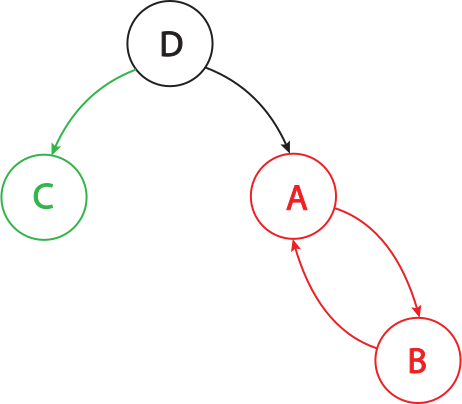
\includegraphics{http://cs241.cs.illinois.edu/images/ColorfulDeadlock.svg}
\caption{}
\end{figure}

\subsection{Coffman conditions}\label{coffman-conditions}

There are four \emph{necessary} and \emph{sufficient} conditions for
deadlock. These are known as the Coffman conditions.

\begin{itemize}
\tightlist
\item
  Mutual Exclusion
\item
  Circular Wait
\item
  Hold and Wait
\item
  No pre-emption
\end{itemize}

If you break any of them, you cannot have deadlock!

All of these conditions are required for deadlock, so let's discuss each
one in turn. First the easy ones- * Mutual Exclusion: The resource
cannot be shared * Circular Wait: There exists a cycle in the Resource
Allocation Graph. There exists a set of processes \{P1,P2,\ldots{}\}
such that P1 is waiting for resources held by P2, which is waiting for
P3,\ldots{}, which is waiting for P1. * Hold and Wait: A process
acquires an incomplete set of resources and holds onto them while
waiting for the other resources. * No pre-emption: Once a process has
acquired a resource, the resource cannot be taken away from a process
and the process will not voluntarily give up a resource.

\subsection{Breaking the Coffman
Conditions}\label{breaking-the-coffman-conditions}

Two students need a pen and paper: * The students share a pen and paper.
Deadlock is avoided because Mutual Exclusion was not required. * The
students both agree to grab the pen before grabbing the paper. Deadlock
is avoided because there cannot be a circular wait. * The students grab
both the pen and paper in one operation (``Get both or get none'').
Deadlock is avoided because there is no \emph{Hold and Wait} * The
students are friends and will ask each other to give up a held resource.
Deadlock is avoided because pre-emption is allowed.

\subsection{Livelock}\label{livelock}

Livelock is \emph{not} deadlock-

Consider the following `solution' * The students will put down one held
resource if they are unable to pick up the other resource within 10
seconds. This solution avoids deadlock however it may suffer from
livelock.

Livelock occurs when a process continues to execute but is unable to
make progress. In practice Livelock may occur because the programmer has
taken steps to avoid deadlock. In the above example, in a busy system,
the student will continually release the first resource because they are
never able to obtain the second resource. The system is not deadlock
(the student process is still executing) however it's not making any
progress either.

\subsection{Deadlock Prevention/Avoidance vs Deadlock
Detection}\label{deadlock-preventionavoidance-vs-deadlock-detection}

Deadlock prevention is making sure that deadlock cannot happen, meaning
that you break a coffman condition. This works the best inside a single
program and the software engineer making the choice to break a certain
coffman condition. Consider the
\href{https://en.wikipedia.org/wiki/Banker's_algorithm}{Banker's
Algorithm}. It is another algorithm for deadlock avoidance. The whole
implementation is outside the scope of this class, just know that there
are more generalized algorithms for operating systems.

Deadlock detection on the other hand is allowing the system to enter a
deadlocked state. After entering, the system uses the information that
it has to break deadlock. As an example, consider multiple processes
accessing files. The operating system is able to keep track of all of
the files/resources through file descriptors at some level (either
abstracted through an API or directly). If the operating system detects
a directed cycle in the operating system file descriptor table it may
break one process' hold (through scheduling for example) and let the
system proceed.

\subsection{Dining Philosophers}\label{dining-philosophers}

The Dining Philosophers problem is a classic synchronization problem.
Imagine I invite N (let's say 5) philosophers to a meal. We will sit
them at a table with 5 chopsticks (one between each philosopher). A
philosopher alternates between wanting to eat or think. To eat the
philosopher must pick up the two chopsticks either side of their
position (the original problem required each philosopher to have two
forks). However these chopsticks are shared with his neighbor.

\begin{figure}[htbp]
\centering
\includegraphics{https://raw.githubusercontent.com/wiki/angrave/SystemProgramming/5DiningPhilosophers.png}
\caption{5DiningPhilosophers}
\end{figure}

Is it possible to design an efficient solution such that all
philosophers get to eat? Or, will some philosophers starve, never
obtaining a second chopstick? Or will all of them deadlock? For example,
imagine each guest picks up the chopstick on their left and then waits
for the chopstick on their right to be free. Oops - our philosophers
have deadlocked!

\section{Backstory}\label{backstory}

So you have your philosophers sitting around a table all wanting to eat
some pasta (or whatever that is) and they are really hungry. Each of the
philosophers are essentially the same, meaning that each philosopher has
the same instruction set based on the other philosopher ie you can't
tell every even philosopher to do one thing and every odd philosopher to
do another thing.

\section{Failed Solutions}\label{failed-solutions}

\subsection{Left-Right Deadlock}\label{left-right-deadlock}

What do we do? Let's try a simple solution

\begin{Shaded}
\begin{Highlighting}[]
\DataTypeTok{void}\NormalTok{* philosopher(}\DataTypeTok{void}\NormalTok{* forks)\{}
     \NormalTok{info phil_info = forks;}
     \NormalTok{pthread_mutex_t* left_fork = phil_info->left_fork;}
     \NormalTok{pthread_mutex_t* right_fork = phil_info->right_fork;}
     \KeywordTok{while}\NormalTok{(phil_info->simulation)\{}
          \NormalTok{pthread_mutex_lock(left_fork);}
          \NormalTok{pthread_mutex_lock(right_fork);}
          \NormalTok{eat(left_fork, right_fork);}
          \NormalTok{pthread_mutex_unlock(left_fork);}
          \NormalTok{pthread_mutex_unlock(right_fork);}
     \NormalTok{\}}
\NormalTok{\}}
\end{Highlighting}
\end{Shaded}

But this runs into a problem! What if everyone picks up their left fork
and is waiting on their right fork? We have deadlocked the program. It
is important to note that deadlock doesn't happen all the time and the
probability that this solution deadlocks goes down as the number of
philosophers goes up. What is really important to note is that
eventually that this solution will deadlock, letting threads starve
which is bad.

\subsection{Trylock? More like
livelock}\label{trylock-more-like-livelock}

So now you are thinking about breaking one of the coffman conditions. We
have - Mutual Exclusion - No Preemption - Hold and wait - Circular Wait

Well we can't have two philosophers use a fork at the same time, mutual
exclusion is out of the picture. In our current, simple model, we can't
have the philosopher let go of the mutex lock once he/she has a hold of
it, so we will take this solution out right now -- there are some notes
at the bottom of the page about this solution. Let's break Hold and
Wait!

\begin{Shaded}
\begin{Highlighting}[]
\DataTypeTok{void}\NormalTok{* philosopher(}\DataTypeTok{void}\NormalTok{* forks)\{}
     \NormalTok{info phil_info = forks;}
     \NormalTok{pthread_mutex_t* left_fork = phil_info->left_fork;}
     \NormalTok{pthread_mutex_t* right_fork = phil_info->right_fork;}
     \KeywordTok{while}\NormalTok{(phil_info->simulation)\{}
          \NormalTok{pthread_mutex_lock(left_fork);}
          \DataTypeTok{int} \NormalTok{failed = pthread_mutex_trylock(right_fork);}
          \KeywordTok{if}\NormalTok{(!failed)\{}
               \NormalTok{eat(left_fork, right_fork);}
               \NormalTok{pthread_mutex_unlock(right_fork);}
          \NormalTok{\}}
          \NormalTok{pthread_mutex_unlock(left_fork);}
     \NormalTok{\}}
\NormalTok{\}}
\end{Highlighting}
\end{Shaded}

Now our philosopher picks up the left fork and tries to grab the right.
If it's available, they eat. If it's not available, they put the left
fork down and try again. No deadlock!

But, there is a problem. What if all the philosophers pick up their left
at the same time, try to grab their right, put their left down, pick up
their left, try to grab their right\ldots{}. We have now livelocked our
solution! Our poor philosopher are still starving, so let's give them
some proper solutions.

\section{Viable Solutions}\label{viable-solutions}

\subsection{Arbitrator (Naive and
Advanced).}\label{arbitrator-naive-and-advanced.}

The naive arbitrator solution is have one arbitrator (a mutex for
example). Have each of the philosopher ask the arbitrator for permission
to eat. This solution allows one philosopher to eat at a time. When they
are done, another philosopher can ask for permission to eat.

This prevents deadlock because there is no circular wait! No philosopher
has to wait on any other philosopher.

The advanced arbitrator solution is to implement a class that determines
if the philosopher's forks are in the arbitrator's possession. If they
are, they give them to the philosopher, let him eat, and take the forks
back. This has the added bonus of being able to have multiple
philosopher eat at the same time.

\subsubsection{Problems:}\label{problems}

\begin{itemize}
\tightlist
\item
  These solutions are slow
\item
  They have a single point of failure, the arbitrator making it a
  bottleneck
\item
  The arbitrator needs to also be fair, and be able to determine
  deadlock in the second solution
\item
  In practical systems, the arbitrator tends to give the forks
  repeatedly to philosophers that just ate because of process scheduling
\end{itemize}

\subsection{Leaving the Table (Stallings'
Solution)}\label{leaving-the-table-stallings-solution}

Why does the first solution deadlock? Well there are n philosophers and
n chopsticks. What if there is only 1 philsopher at the table? Can we
deadlock? No.

How about 2 philsophers? 3? \ldots{} You can see where this is going.
Stallings' solutions says to remove philosophers from the table until
deadlock is not possible -- think about what the magic number of
philosophers at the table is. The way to do this in actual system is
through semaphores and letting a certain number of philosopher through.

\subsubsection{Problems:}\label{problems-1}

\begin{itemize}
\tightlist
\item
  The solution requires a lot of context switching which is very
  expensive for the CPU
\item
  You need to know about the number of resources before hand in order to
  only let that number of philosophers
\item
  Again priority is given to the processes who have already eaten.
\end{itemize}

\subsection{Partial Ordering (Dijkstra's
Solution)}\label{partial-ordering-dijkstras-solution}

This is Dijkstra's solution (he was the one to propose this problem on
an exam). Why does the first solution deadlock? Dijkstra thought that
the last philosopher who picks up his left fork (causing the solution to
deadlock) should pick up his right. He accomplishes it by number the
forks 1..n, and tells each of the philosopher to pick up his lower
number fork.

Let's run through the deadlock condition again. Everyone tries to pick
up their lower number fork first. Philosopher 1 gets fork 1, Philosopher
2 gets fork 2, and so on until we get to Philosopher n. They have to
choose between fork 1 and n. fork 1 is already held up by philosopher 1,
so they can't pick up that fork, meaning he won't pick up fork n. We
have broken circular wait! Meaning deadlock isn't possible.

\subsubsection{Problems:}\label{problems-2}

\begin{itemize}
\tightlist
\item
  The philosopher needs to know the set of resources in order before
  grabbing any resources.
\item
  You need to define a partial order to all of the resources.
\item
  Prioritizes philosopher who have already eaten.
\end{itemize}

\subsection{Advanced Solutions}\label{advanced-solutions}

There are many more advanced solutions a non-exhaustive list includes -
Clean/Dirty Forks (Chandra/Misra Solution) - Actor Model (other Message
passing models) - Super Arbitrators (Complicated pipelines)

\section{Topics}\label{topics}

Coffman Conditions Resource Allocation Graphs Dining Philosophers *
Failed DP Solutions * Livelocking DP Solutions * Working DP Solutions:
Benefits/Drawbacks

\section{Questions}\label{questions}

\begin{itemize}
\item
  What are the Coffman Conditions?
\item
  What do each of the Coffman conditions mean? (e.g.~can you provide a
  definition of each one)
\item
  Give a real life example of breaking each Coffman condition in turn. A
  situation to consider: Painters, Paint, Paintbrushes etc. How would
  you assure that work would get done?
\item
  Be able to identify when Dining Philosophers code causes a deadlock
  (or not). For example, if you saw the following code snippet which
  Coffman condition is not satisfied?

\begin{Shaded}
\begin{Highlighting}[]
\CommentTok{// Get both locks or none.}
\NormalTok{pthread_mutex_lock( a );}
\KeywordTok{if}\NormalTok{( pthread_mutex_trylock( b ) ) \{ }\CommentTok{/*failed*/}
   \NormalTok{pthread_mutex_unlock( a );}
   \NormalTok{...}
\NormalTok{\}}
\end{Highlighting}
\end{Shaded}
\item
  If one thread calls

\begin{Shaded}
\begin{Highlighting}[]
  \NormalTok{pthread_mutex_lock(m1) }\CommentTok{// success}
  \NormalTok{pthread_mutex_lock(m2) }\CommentTok{// blocks}
\end{Highlighting}
\end{Shaded}

  and another threads calls

\begin{Shaded}
\begin{Highlighting}[]
  \NormalTok{pthread_mutex_lock(m2) }\CommentTok{// success}
  \NormalTok{pthread_mutex_lock(m1) }\CommentTok{// blocks}
\end{Highlighting}
\end{Shaded}

  What happens and why? What happens if a third thread calls
  \texttt{pthread\_mutex\_lock(m1)} ?
\item
  How many processes are blocked? As usual assume that a process is able
  to complete if it is able to acquire all of the resources listed
  below.

  \begin{itemize}
  \tightlist
  \item
    P1 acquires R1
  \item
    P2 acquires R2
  \item
    P1 acquires R3
  \item
    P2 waits for R3
  \item
    P3 acquires R5
  \item
    P1 waits for R4
  \item
    P3 waits for R1
  \item
    P4 waits for R5
  \item
    P5 waits for R1
  \end{itemize}
\end{itemize}

(Draw out the resource graph!)
